
\documentclass{article}
\usepackage[landscape]{geometry}
\usepackage{url}
\usepackage{multicol}
\usepackage{amsmath}
\usepackage{esint}
\usepackage{amsfonts}
\usepackage{tikz}
\usetikzlibrary{decorations.pathmorphing}
\usepackage{amsmath,amssymb}

\usepackage{colortbl}
\usepackage{xcolor}
\usepackage{mathtools}
\usepackage{amsmath,amssymb}
\usepackage{enumitem}
\makeatletter

\newcommand*\bigcdot{\mathpalette\bigcdot@{.5}}
\newcommand*\bigcdot@[2]{\mathbin{\vcenter{\hbox{\scalebox{#2}{$\m@th#1\bullet$}}}}}
\makeatother

\title{130 Cheat Sheet}
\usepackage[brazilian]{babel}
\usepackage[utf8]{inputenc}

\advance\topmargin-1in
\advance\textheight3in
\advance\textwidth3in
\advance\oddsidemargin-1.5in
\advance\evensidemargin-1.5in
\parindent0pt
\parskip2pt
\newcommand{\hr}{\centerline{\rule{3.5in}{1pt}}}
%\colorbox[HTML]{e4e4e4}{\makebox[\textwidth-2\fboxsep][l]{texto}
\begin{document}

\begin{center}{\huge{\textbf{Classical Mechanics}}}\\
\end{center}
\begin{multicols*}{3}

\tikzstyle{mybox} = [draw=black, fill=white, very thick,
    rectangle, rounded corners, inner sep=10pt, inner ysep=10pt]
\tikzstyle{fancytitle} =[fill=white, text=black, font=\bfseries]

%------------  ---------------
\begin{tikzpicture}
\node [mybox] (box){%
    \begin{minipage}{0.3\textwidth}
%$$
%x(t)=v_{0 x} t+x_0, \quad y(t)=-\frac{1}{2} g t^2+v_{0 y} t+y_0
%$$
%$$
%v_f^2-v_i^2=2 a \Delta x
%$$
Equations of Motion for \textbf{Constant Linear Acceleration}\\
\[
\begin{aligned}
&\begin{array}{cl}
\hline \text{Linear Equation} & \text{Missing Variable} \\
\hline v=v_0+at & x-x_0 \\
x-x_0=v_0 t+\frac{1}{2} a t^2 & v \\
x-x_0=\frac{1}{2}(v_0+v)t & a \\
v^2=v_0^2+2a(x-x_0) & t \\
x-x_0=vt-\frac{1}{2} a t^2 & v_0 \\
\hline
\end{array}
\end{aligned}
\]
Equations of Motion for \textbf{Constant Angular Acceleration}
\[
\begin{aligned}
&\begin{array}{cl}
\hline \text{Angular Equation} & \text{Missing Variable} \\
\hline \omega=\omega_0+\alpha t & \theta-\theta_0 \\
\theta-\theta_0=\omega_0 t+\frac{1}{2} \alpha t^2 & \omega \\
\theta-\theta_0=\frac{1}{2}(\omega_0+\omega)t & \alpha \\
\omega^2=\omega_0^2+2\alpha(\theta-\theta_0) & t \\
\theta-\theta_0=\omega t-\frac{1}{2} \alpha t^2 & \omega_0 \\
\hline
\end{array}
\end{aligned}
\]

    \end{minipage}
};
%------------ Kinematics Header ---------------------
\node[fancytitle, right=10pt] at (box.north west) {Kinematics};
\end{tikzpicture}

%------------ Rotational Motion ---------------
\begin{tikzpicture}
\node [mybox] (box){%
    \begin{minipage}{0.3\textwidth}
    \begin{itemize}
        \item Rotational angle $\theta$
    \end{itemize}
    $$
\theta=\frac{s}{r} \quad \text { (radian measure) }
$$
where $s$ is the arc length of a circular path of radius $r$ and angle $\theta$.
%$$
\begin{itemize}
    \item Angular velocity $\omega$ (instantaneous)
\end{itemize}
$$
\omega=\frac{d \theta}{d t} .
$$
$\omega$ is a vector, with directions given by a right-hand rule. They are positive for counterclockwise rotation.
\begin{itemize}
    \item Angular acceleration $\alpha$ (instantaneous)
\end{itemize}
$$
\alpha=\frac{d \omega}{d t} .
$$
    \end{minipage}
};
%------------ Rotational Motion Header ---------------------
\node[fancytitle, right=10pt] at (box.north west) {Rotational Motion};
\end{tikzpicture}


%------------ Relation between linear and angular variables Motion ---------------
\begin{tikzpicture}
\node [mybox] (box){%
    \begin{minipage}{0.3\textwidth}
%A point in a rigid rotating body, at a perpendicular distance $r$ from the rotation axis, moves in a circle with radius $r$. 
In case of rolling without slipping. 
If the body rotates through an angle $\theta$, the point moves along an arc with length $s$ given by
$$
s=\theta r \quad \text { (radian measure), }
$$
%where $\theta$ is in radians.
The linear velocity $\vec{v}$ 
%of the point 
is tangent to the circle; the point's linear speed $v$ is given by
$$
v=\omega r \quad \text { (radian measure), }
$$
where $\omega$ is the angular speed (in radians per second).\\
%of the body, and thus also the point.
The linear acceleration $\vec{a}$ of the point has both tangential and radial components. The tangential component is
$$
a_t=\alpha r \quad \text { (radian measure), }
$$
where $\alpha$ is the magnitude of the angular acceleration (in radians per second-squared)
%of the body. 
The radial component of $\vec{a}$ is
$$
a_r=\frac{v^2}{r}=\omega^2 r \quad \text { (radian measure). }
$$
If the point moves in uniform circular motion, the tangential acceleration is zero so the force will be 
$$
F= m a_r = \frac{m v^2}{r}
$$
the period $T$ of the motion is 
$$
T=\frac{2 \pi r}{v}=\frac{2 \pi}{\omega} \quad \text { (radian measure). }
$$
    \end{minipage}
};

%------------ Relation between linear and angular variables Header ---------------------
\node[fancytitle, right=10pt] at (box.north west) {Relation between linear and angular variables};
\end{tikzpicture}

%------------  Moment of Inertia Content ---------------
\begin{tikzpicture}
\node [mybox] (box){%
    \begin{minipage}{0.3\textwidth}
An object's moment of inertia is analogous to its mass in the context of rotation, but, unlike mass, it depends on the distance from the center of rotation. Let's start with a point particle of mass $m$ : the moment of inertia scales with the radius as
$$
I=m r^2
$$

We can generalize to extended objects with arbitrary mass distributions by integrating:
$$
I=\int r^2 d m
$$
\textbf{Parallel-axis theorem:}
If we know the moment of inertia $I$ of a system of mass $M$ rotating about an axis through its center of mass (CM), then its moment of inertia about any axis parallel to the $\mathrm{CM}$ axis is given by
$$
I=I_{\mathrm{CM}}+M h^2,
$$
Where h is the distance between the CM axis and the parallel axis.
    \end{minipage}
};
%------------  Moment of Inertia Header ---------------------
\node[fancytitle, right=10pt] at (box.north west) { Moment of Inertia};
\end{tikzpicture}















%------------ Energy ---------------
\begin{tikzpicture}
\node [mybox] (box){%
    \begin{minipage}{0.3\textwidth}
\textit{If an object is acted on only by conservative forces, the sum of its kinetic and potential energies is constant along the object’s path.}\\\\
You should know the following formulas cold:
$$
\begin{aligned}
&\text { Translational kinetic energy: }  \frac{1}{2} m v^2 \\
&\text { Rotational kinetic energy: }  \frac{1}{2} I \omega^2 \\
&\text { Gravitational potential energy on Earth: }  m g h \\
&\text { Spring potential energy: }  \frac{1}{2} k x^2
\end{aligned}
$$

$$
\mathbf{F}_{\text {grav }}=\frac{G m_1 m_2}{r^2} \hat{\mathbf{r}}
$$

For any conservative force $\mathbf{F}$, the change in potential energy $\Delta U$ between points $a$ and $b$ is
$$
\Delta U=-\int_a^b \mathbf{F} \cdot d \mathbf{l}
$$
$$
\mathbf{F}=-\nabla U
$$
    \end{minipage}
};
%------------ Energy Header ---------------------
\node[fancytitle, right=10pt] at (box.north west) {Energy};
\end{tikzpicture}

%------------ Rolling Without Slipping ---------------
\begin{tikzpicture}
\node [mybox] (box){%
    \begin{minipage}{0.3\textwidth}
If the object (sphere, cylinder, and so forth) rolls without slipping, then its linear velocity $v$ and angular velocity $\omega$ are related by
$$
v_{com}=R \omega,
$$
    \end{minipage}
};
%------------ Rolling Without Slipping ---------------------
\node[fancytitle, right=10pt] at (box.north west) {Rolling Without Slipping};
\end{tikzpicture}
%------------ Work–Energy Theorem Content ---------------------
\begin{tikzpicture}
\node [mybox] (box){%
    \begin{minipage}{0.3\textwidth}
    To quantify the effects of nonconservative forces such as friction: 
$$
E_{\text {initial }}+W_{\text {other }}=E_{\text {final }} \text {, }
$$
where $W_{\text {other }}$ is the work due to nonconservative forces.
$$
W=\Delta \mathrm{KE}
$$
Here W is the work done by all forces, including the conservative ones. \\\\
The general definition of work:
$$
W=\int \mathbf{F} \cdot d \mathbf{l}
$$
    \end{minipage}
};
%------------ Work–Energy Theorem Header ---------------------
\node[fancytitle, right=10pt] at (box.north west) {Work–Energy Theorem};
\end{tikzpicture}

%------------ Momentum Content ---------------
\begin{tikzpicture}
\node [mybox] (box){%
    \begin{minipage}{0.3\textwidth}
\textit{Momentum is always conserved in a system in the absence of external forces.}
$$
\mathbf{p}=m \mathbf{v} \text { and } \mathbf{F}=d \mathbf{p} / d t
$$
    \end{minipage}
};
%------------ Momentum Header ---------------------
\node[fancytitle, right=10pt] at (box.north west) {Momentum};
\end{tikzpicture}

%------------ Rotational Motion and Angular Momentum Content ---------------
\begin{tikzpicture}
\node [mybox] (box){%
    \begin{minipage}{0.3\textwidth}
The angular momentum of a point particle of linear momentum $\mathbf{p}$ is defined by
$$
\mathbf{L}=\mathbf{r} \times \mathbf{p}
$$
For an extended body we also have
$$
\mathbf{L}=I \boldsymbol{\omega},
$$
Extending the metaphor, the analogue of force F for rotational motion is the torque:
$$
\boldsymbol{\tau}=\mathbf{r} \times \mathbf{F}
$$
second law $F=m a$ at the price of introducing "fictitious" forces, which only appear because of the noninertial choice of coordinates:
$$
\begin{aligned}
F_{\text {centrifugal }} & =-m \Omega^2 r, \\
F_{\text {Coriolis }} & =-2 m \boldsymbol{\Omega} \times \mathbf{v} .
\end{aligned}
$$
    \end{minipage}
};
%------------ Rotational Motion and Angular Momentum Header ---------------------
\node[fancytitle, right=10pt] at (box.north west) {Rotational Motion and Angular Momentum};
\end{tikzpicture}

%------------ Center of Mass Content ---------------
\begin{tikzpicture}
\node [mybox] (box){%
    \begin{minipage}{0.3\textwidth}
$\mathbf{r}_{\mathrm{CM}}=\frac{\int \mathbf{r} d m}{M}$ and 
$\mathbf{r}_{\mathrm{CM}}=\frac{\sum_i \mathbf{r}_i m_i}{M}$
    \end{minipage}
};
%------------ Center of Mass Header ---------------------
\node[fancytitle, right=10pt] at (box.north west) {Center of Mass};
\end{tikzpicture}
\
%------------ Lagrangians Content ---------------
\begin{tikzpicture}
\node [mybox] (box){%
    \begin{minipage}{0.3\textwidth}
The Lagrangian $L$ of a system is a scalar function described by this simple formula:
$$
L(q, \dot{q}, t)=T-U
$$
\begin{itemize}
    \item Write down expressions for the Cartesian coordinates in terms of your chosen coordinates $q$.
    \item  Differentiate the Cartesian coordinates $(x, y, z)$ with respect to time to get $(\dot{x}, \dot{y}, \dot{z})$, paying careful attention to the chain rule.
    \item Form the expression for the Cartesian kinetic energy, $T=$ $\frac{1}{2} m\left(\dot{x}^2+\dot{y}^2+\dot{z}^2\right)$ for a point particle or $T=\frac{1}{2} I \omega^2$ for an extended object, as appropriate. For the latter, you'll need to express $\omega$ in terms of the velocities $\dot{q}$, but this is typically easy because you will have chosen coordinates such that $\dot{q}$ is $\omega$.
\end{itemize}
    \end{minipage}
};
%------------ Lagrangians Header ---------------------
\node[fancytitle, right=10pt] at (box.north west) {Lagrangians};
\end{tikzpicture}
%------------ Euler–Lagrange Equations Content ---------------------
\begin{tikzpicture}
\node [mybox] (box){%
    \begin{minipage}{0.3\textwidth}
The Lagrangian equations of motion, or more commonly, the Euler-Lagrange equations,
$$
\frac{d}{d t} \frac{\partial L}{\partial \dot{q}}=\frac{\partial L}{\partial q}
$$
$$
p_i \equiv \frac{\partial L}{\partial \dot{q}}: \text { momentum conjugate to } q \text {. }
$$
	\end{minipage}
};
%------------ Euler–Lagrange Equations Header ---------------------
\node[fancytitle, right=10pt] at (box.north west) {Euler–Lagrange Equations};
\end{tikzpicture}

%------------ Hamiltonians and Hamilton’s Equations of Motion Content ---------------------
\begin{tikzpicture}
\node [mybox] (box){%
    \begin{minipage}{0.3\textwidth}
$$
H(p, q)=\sum_i p_i \dot{q}_i-L
$$
$H=T+U \quad$ (if $U$ does not depend explicitly on velocities or time).\\\\
As opposed to the second-order Euler-Lagrange equations. These are Hamilton's equations:
$$
\dot{p}=-\frac{\partial H}{\partial q}, \quad \dot{q}=\frac{\partial H}{\partial p}
$$
	\end{minipage}
};
%------------ Hamiltonians and Hamilton’s Equations of Motion Header ---------------------
\node[fancytitle, right=10pt] at (box.north west) {Hamiltonians and Hamilton’s Equations of Motion};
\end{tikzpicture}



%------------  Springs and Harmonic Oscillators ---------------
\begin{tikzpicture}
\node [mybox] (box){%
    \begin{minipage}{0.3\textwidth}
    Hooke’s law
$$
F=m \ddot{x}=-k x
$$
This is an ordinary differential equation describing a harmonic oscillator whose solutions are of the form $\boxed{x(t)=A \cos (\omega t+\phi)}$. The angular frequency is given by
$$
\omega=\sqrt{\frac{k}{m}} .
$$
Note that the amplitude $A$ is not determined by Hooke's law, but is instead a constant of integration fixed by the initial conditions. The phase $\phi$ is the second constant of integration.

$\boxed{x(t)=A e^{i \omega t}}$,
with A allowed to be complex, also satisfy Hooke’s law.\\
The potential energy of a spring of a constant k:
$$U=\frac{1}{2} k x^2$$

Correspondence of quantities in the analogy between electrical and mechanical systems.
\begin{tabular}{lll}
\hline Mechanical system & Circuit system \\
\hline$x$ displacement & $q$ charge \\
$\dot{x}$ velocity & $I$ current \\
$m$ mass & $L$ inductance \\
$b$ damping resistance & $R$ electrical resistance \\
$1 / k$ spring stiffness & $C$ capacitance \\
$F$ amplitude  & $V$ amplitude  \\
of driving force & of driving voltage \\
\hline
\end{tabular}
    \end{minipage}
};

%------------  Springs and Harmonic Oscillators Header ---------------------
\node[fancytitle, right=10pt] at (box.north west) {Springs and Harmonic Oscillators};
\end{tikzpicture}


%------------  Bernoulli’s Principle ---------------
\begin{tikzpicture}
\node [mybox] (box){%
    \begin{minipage}{0.3\textwidth}
    \textit{Bernoulli’s Principle is a key concept in fluid dynamics that relates pressure, speed and height. Bernoulli's principle states that an increase in the speed of a fluid occurs simultaneously with a decrease in static pressure or the fluid's potential energy}
$$
\frac{v^2}{2}+g z+\frac{p}{\rho}=\text { constant }
$$
    \centering
    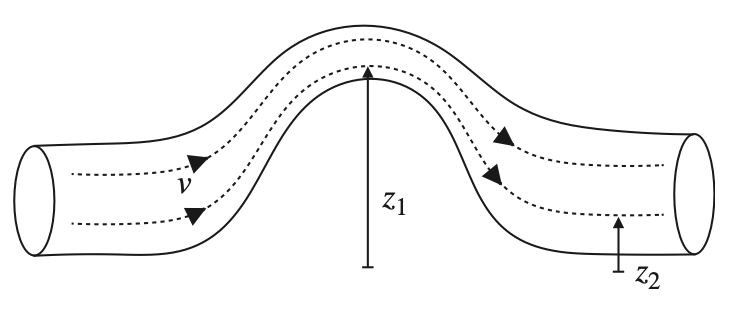
\includegraphics[width=0.8\linewidth]{Bernouli's principle.png}
    \end{minipage}
};

%------------  Bernoulli’s Principle Header ---------------------
\node[fancytitle, right=10pt] at (box.north west) { Bernoulli’s Principle};
\end{tikzpicture}

%------------  Buoyant Forces ---------------
\begin{tikzpicture}
\node [mybox] (box){%
    \begin{minipage}{0.3\textwidth}
    \textit{The upward buoyant force that is exerted on a body immersed in a fluid, whether partially or fully submerged, is equal to the weight of the fluid that the body displaces and acts in the upward direction at the center of mass of the displaced fluid}
$$
F=\rho V g
$$
    \centering
    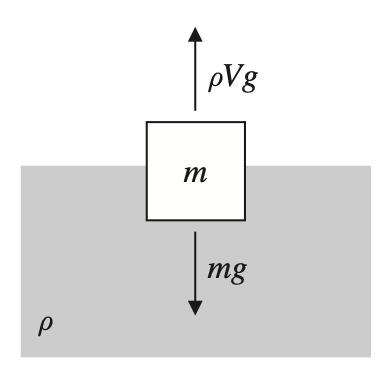
\includegraphics[width=0.5\linewidth]{buoyantforce.png}
    \end{minipage}
};

%------------  Buoyant Forces Header ---------------------
\node[fancytitle, right=10pt] at (box.north west) {Archimedes principle (buoyant forces)};
\end{tikzpicture}

%------------  pascal's principle ---------------
\begin{tikzpicture}
\node [mybox] (box){%
    \begin{minipage}{0.3\textwidth}
    \textit{A change in pressure at any point in an enclosed incompressible fluid at rest is transmitted equally and undiminished to all points in all directions throughout the fluid, and acts at right angles to the enclosing walls.}
$$
F=\frac{P}{A}
$$
    \centering
    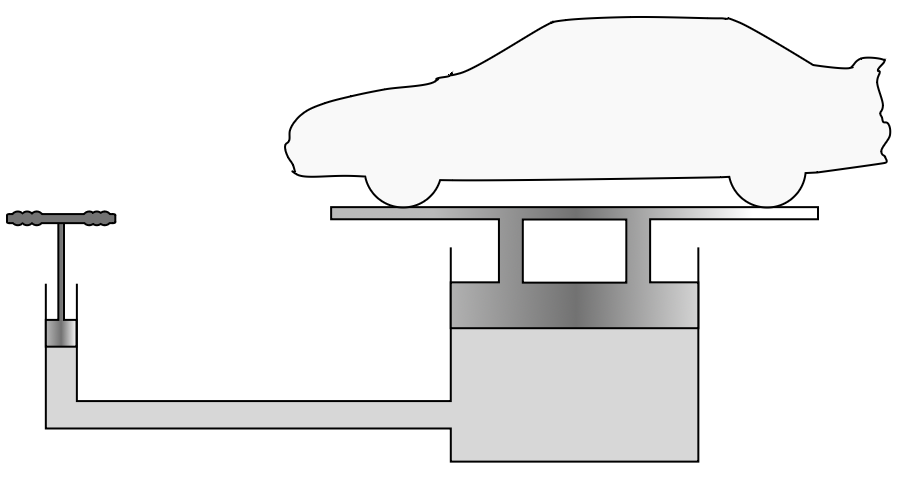
\includegraphics[width=0.5\linewidth]{pascal's principle.png}
    \end{minipage}
};

%------------ pascal's principle Header ---------------------
\node[fancytitle, right=10pt] at (box.north west) {Pascal's principle};
\end{tikzpicture}

\end{multicols*}
\end{document}


Contact GitHub API Training Shop Blog About
© 2016 GitHub, Inc. Terms Privacy Security Status Help